% 2018.01.08 Modified
% 2015.07.10 Modified
%
% mthesis.tex
%
%\documentclass[12pt]{jarticle} % Japanese
\documentclass[12pt]{article} % English
% if there are problems in the above regarding fonts, use this
% \documentclass[UTF8]{ctexart}

\usepackage[utf8]{inputenc}
%\usepackage{utf}
%\usepackage{naist-jmthesis} %Japanese
\usepackage{naist-mthesis} %English

\usepackage{graphicx}

%
% Page style
%
\pagestyle{final}       % Camera-Ready
%\pagestyle{draft}      % Draft
%
%
\lang{Japanese} % Japanese
%\lang{English} % English
%
% Student Number
%
\studentnumber{1911253}
%
% 修士論文 か 課題研究 かの選択
%
\doctitle{\mastersthesis}       % 修士論文
%\doctitle{\mastersreport}      % 課題研究
%
% 取得予定の修士号は 修士(工学) か 修士(理学) か ?
%
\major{\engineering}    % 工学
%\major{\science}       % 理学
%
% 日本語題目 (in LaTeX)
%
\title{ボランティアコンピューティングによるクラウドゲーミングシステム}
%
% 日本語題目 (in plain text)
%
%   注: (in LaTeX)と同じ場合は指定する必要なし。
%       この情報は修士論文/課題研究には現れませんが、管理のために必要です。
%
\ptitle{太陽と月を利用したpiの低速計算アルゴリズムに関する理論的研究}
%
% 英語題目 (in LaTeX)
%
\etitle{Cloud Gaming System by Volunteer Computing}
%
% 英語題目 (in plain text)
%
%   注: (in LaTeX)と同じ場合は指定する必要なし。
%       この情報は修士論文/課題研究には現れませんが、管理のために必要です。
%
\eptitle{Theoretical Studies on Low-Speed Calculation Algorithms of pi \\
Utilizing the Sun and the Moon}
%
% 日本語氏名 (in LaTeX)
%   (姓と名の間に空白を入れて下さい)
%
\author{前田 健登}
%
% 日本語氏名 (in plain text)
%
%   注: (in LaTeX)と同じ場合は指定する必要なし。
%       この情報は修士論文/課題研究には現れませんが、管理のために必要です。
%
\pauthor{}
%
% 欧文氏名 (in LaTeX)
%   (first name, last name の順に記入し、先頭文字のみを大文字にする。)
%
\eauthor{Kento Maeda}
% 別の例: \eauthor{Kurt G\"{o}del}
%
%
% 欧文氏名 (in plain text)
%
%   注: (in LaTeX)と同じ場合は指定する必要なし。
%       この情報は修士論文/課題研究には現れませんが、管理のために必要です。
%
\epauthor{}
% 別の例: \peauthor{Kurt Goedel}
%
%
% 論文提出年月日
%
\syear{2021}
\smonth{1}
\sday{25}
%
% 専攻の選択
%
%\department{\infproc}  % 情報処理学
%\department{\infsys}    % 情報システム学
%\department{\bioinf}   % 情報生命科学
\department{\infsci}    % 情報科学
%
%
% 審査委員(日本語)
%   (姓と名、名と称号の間に空白を入れて下さい)
%
%5人以上の場合,5人目以降は\addcmembers を使って宣言する。
%最大で合わせて8人まで宣言可能。
%主指導教員、副指導教員を明記する。両指導教員以外は委員。
%学外審査委員は、大学名を明記する
%
% 4人の場合
\cmembers{飯田 元 教授}{(主指導教員)}
         {藤川 和利 教授}{(副指導教員)}
         {市川 昊平 准教授}{(副指導教員)}
         {髙橋 慧智 准教授}{(副指導教員)}
%
% 3人の場合
%\cmembers{○○ ○○ 教授}{(主指導教員)}
%         {○○ ○○ 教授}{(副指導教員)}
%         {○○ ○○ 准教授}{(副指導教員)}
%         {}{}
%
% 2人の場合
%\cmembers{○○ ○○ 教授}{(主指導教員)}
%         {○○ ○○ 教授}{(副指導教員)}
%          {}{}
%          {}{}
%
% 5人目の宣言
%\addcmembers{55 55 准教授}{(□□大学)}
%            {}{}
%            {}{}
%            {}{}
%
% 5〜6人目の宣言
%\addcmembers{55 55 准教授}{(□□大学)}
%            {66 66 准教授}{(□□大学)}
%            {}{}
%            {}{}
%
% 5〜7人目の宣言
%\addcmembers{55 55 准教授}{(□□大学)}
%            {66 66 准教授}{(□□大学)}
%            {77 77 准教授}{(□□大学)}
%            {}{}
%
% 5〜8人目の宣言
%\addcmembers{55 55 准教授}{(□□大学)}
%            {66 66 准教授}{(□□大学)}
%            {77 77 准教授}{(□□大学)}
%            {88 88 准教授}{(□□大学)}
%
%
% 審査委員(英語)
%     (first name, last name の順に記入し、先頭文字のみを大文字にする。
%       first name と last name の間に空白、
%       last name と 称号の間にカンマと空白を入れて下さい。)
%
% 5人以上の場合,5人目以降は\eaddcmembers を使って宣言する
% Supervisor, Co-supervisor, and Member must be specified.
% 4人の場合
\ecmembers{Professor Hajimu Iida}{(Supervisor)}
          {Professor Kazutoshi Fujikawa}{(Co-supervisor)}
          {Associate Professor Kouhei Ichikawa}{(Co-supervisor)}
          {Assistant Professor Keichi Takahashi}{(Co-supervisor)}
%
% 3人の場合
%\ecmembers{Professor XXX XXX}{(Supervisor)}
%          {Professor XXX XXX}{(Co-supervisor)}
%          {Associate Professor XXX XXX}{(Co-supervisor)}
%          {}{}
%
% 2人の場合
% \ecmembers{Professor XXX XXX}{(Supervisor)}
%           {Professor XXX XXX}{(Co-supervisor)}
%           {}{}
%           {}{}
%
% 5人目の宣言
%\eaddcmembers{Professor 55 55}{(YY University)}
%            {}{}
%            {}{}
%            {}{}
%
% 5〜6人目の宣言
%\eaddcmembers{Professor 55 55}{(YY University)}
%             {Professor 66 66}{(YY University)}
%             {}{}
%             {}{}
%
% 5〜7人目の宣言
%\eaddcmembers{Professor 55 55}{(YY University)}
%             {Professor 66 66}{(YY University)}
%             {Professor 77 77}{(YY University)}
%             {}{}
%
% 5〜8人目の宣言
%\eaddcmembers{Professor 55 55}{(YY University)}
%             {Professor 66 66}{(YY University)}
%             {Professor 77 77}{(YY University)}
%             {Professor 88 88}{(YY University)}
%
%
%
% キーワード5〜6個 (in LaTeX)
%
\keywords{ネットワーク,クラウド,クラウドゲーミング,ボランティアコンピューティング}
%
% キーワード5〜6個 (in plain text)
%
%   注: (in LaTeX)と同じ場合は記入する必要なし。
%       この情報は修士論文/課題研究には現れませんが、管理のために必要です。
%
\pkeywords{pi, 天文学, 数学, 計算機, アルゴリズム}
%
% 5 or 6 Keywords (in LaTeX)
%
\ekeywords{network, cloud, cloud gaming, volunteer computing}
%
% 5 or 6 Keywords (in plain text)
%
%   注: (in LaTeX)と同じ場合は記入する必要なし。
%       この情報は修士論文/課題研究には現れませんが、管理のために必要です。
%
\epkeywords{pi, astronomy, mathematics, computer, algorithm}
%
% 内容梗概 (in LaTeX)
%
%   注: 行の先頭が\\で始まらないようにすること。
%
\abstract{
人類がこの地上に現われて以来、$\pi$の計算には多くの関心が払われてきた。

本論文では、太陽と月を利用して$\pi$を低速に計算するための
画期的なアルゴリズムを与える。

ここには内容梗概を書く。ここには内容梗概を書く。ここには内容梗概を書く。
ここには内容梗概を書く。ここには内容梗概を書く。ここには内容梗概を書く。
ここには内容梗概を書く。ここには内容梗概を書く。ここには内容梗概を書く。
ここには内容梗概を書く。ここには内容梗概を書く。ここには内容梗概を書く。
ここには内容梗概を書く。ここには内容梗概を書く。ここには内容梗概を書く。

ここには内容梗概を書く。ここには内容梗概を書く。ここには内容梗概を書く。
ここには内容梗概を書く。ここには内容梗概を書く。ここには内容梗概を書く。
ここには内容梗概を書く。ここには内容梗概を書く。ここには内容梗概を書く。
ここには内容梗概を書く。ここには内容梗概を書く。ここには内容梗概を書く。
ここには内容梗概を書く。ここには内容梗概を書く。ここには内容梗概を書く。
}
%
% 内容梗概 (in plain text)
%
%   注: (in LaTeX)と同じ場合は記入する必要なし。
%       この情報は修士論文/課題研究には現れませんが、管理のために必要です。
%       改行する箇所には空白行を入れる。
%       行の先頭が\\で始まらないようにすること。
%
\pabstract{
人類がこの地上に現われて以来、piの計算には多くの関心が払われてきた。

本論文では、太陽と月を利用してpiを低速に計算するための
画期的なアルゴリズムを与える。
}
%
% Abstract (in LaTeX)
%
%  注:  行の先頭が\\で始まらないようにすること。
%
\eabstract{
The calculation of $\pi$ has been paid much attention since human beings
appeared on the earth.

This thesis presents novel low-speed algorithms to calculate
$\pi$ utilizing the sun and the moon.

This is a sample abstract. This is a sample abstract. 
This is a sample abstract. This is a sample abstract. 
This is a sample abstract. This is a sample abstract. 
This is a sample abstract. This is a sample abstract. 
This is a sample abstract. This is a sample abstract. 

This is a sample abstract. This is a sample abstract. 
This is a sample abstract. This is a sample abstract. 
This is a sample abstract. This is a sample abstract. 
This is a sample abstract. This is a sample abstract. 
This is a sample abstract. This is a sample abstract. 
}
%
% Abstract (in plain text)
%
%   注: (in LaTeX)と同じ場合は記入する必要なし。
%       この情報は修士論文/課題研究には現れませんが、管理のために必要です。
%       改行する箇所には空白行を入れる。
%       行の先頭が\\で始まらないようにすること。
%
\epabstract{
The calculation of pi has been paid much attention since human beings
appeared on the earth.

This thesis presents novel low-speed algorithms to calculate
pi utilizing the sun and the moon.
}
%%%%%%%%%%%%%%%%%%%%%%%%% document starts here %%%%%%%%%%%%%%%%%%%%%%%%%%%%
\begin{document}
%
% 表紙 および アブストラクト
%
\titlepage
\cmemberspage
\firstabstract
\secondabstract
%
% 目次
%
\toc
\newpage
\listoffigures
%\newpage
\listoftables
%
% これ以降本文
%
\newpage
\section{はじめに}
ゲーム産業は娯楽産業の中でも大きな収益を上げている産業であり、2019年の世界ゲームコンテンツ市場の規模は15兆6898億円と推定されている\cite{prtimes}。国内でも10年連続で成長しており、市場規模は1兆7330億円となっている。その中でも家庭用ハードや家庭用ソフトと比較して、スマートフォンのアプリやPC向けのオンラインゲームなどといったオンラインプラットフォームのゲームの市場規模が年々大きく拡大している。このようにゲームのプレイスタイルがゲーム専用のハードを購入するというものから汎用デバイスでのゲームプレイへと変化を見せている。こういった状況下で注目されている新たな手法で展開されるゲームサービスの一つにクラウドゲーミングがある。

従来のゲームプレイは、プレイヤーがゲーム専用ハードやゲーミングPC等を所有し、その上でゲームを動作させることによって実現されている。一方、クラウドゲーミングというサービスにおいては、図\ref{fig:cloudgaming}のようにクラウドサーバ上でゲームを動作させてその画面をクライアントであるプレイヤーの端末にストリーミングすることで、ゲームをネットワーク越しにプレイすることを可能にしている。このとき、プレイヤーがゲームプレイに使用する端末は、クラウドサーバより送信されるゲーム画面の再生とプレイヤーの操作のサーバへの送信だけを行う。この仕組みによって、スマートフォンやタブレット端末等の性能が貧弱なデバイスでも、従来は高価なゲームハードやゲーミングPCを使用しなければ体験できなかったような高品質なゲーム体験を得られることが期待されている。

\begin{figure*}[t]
    \centering
    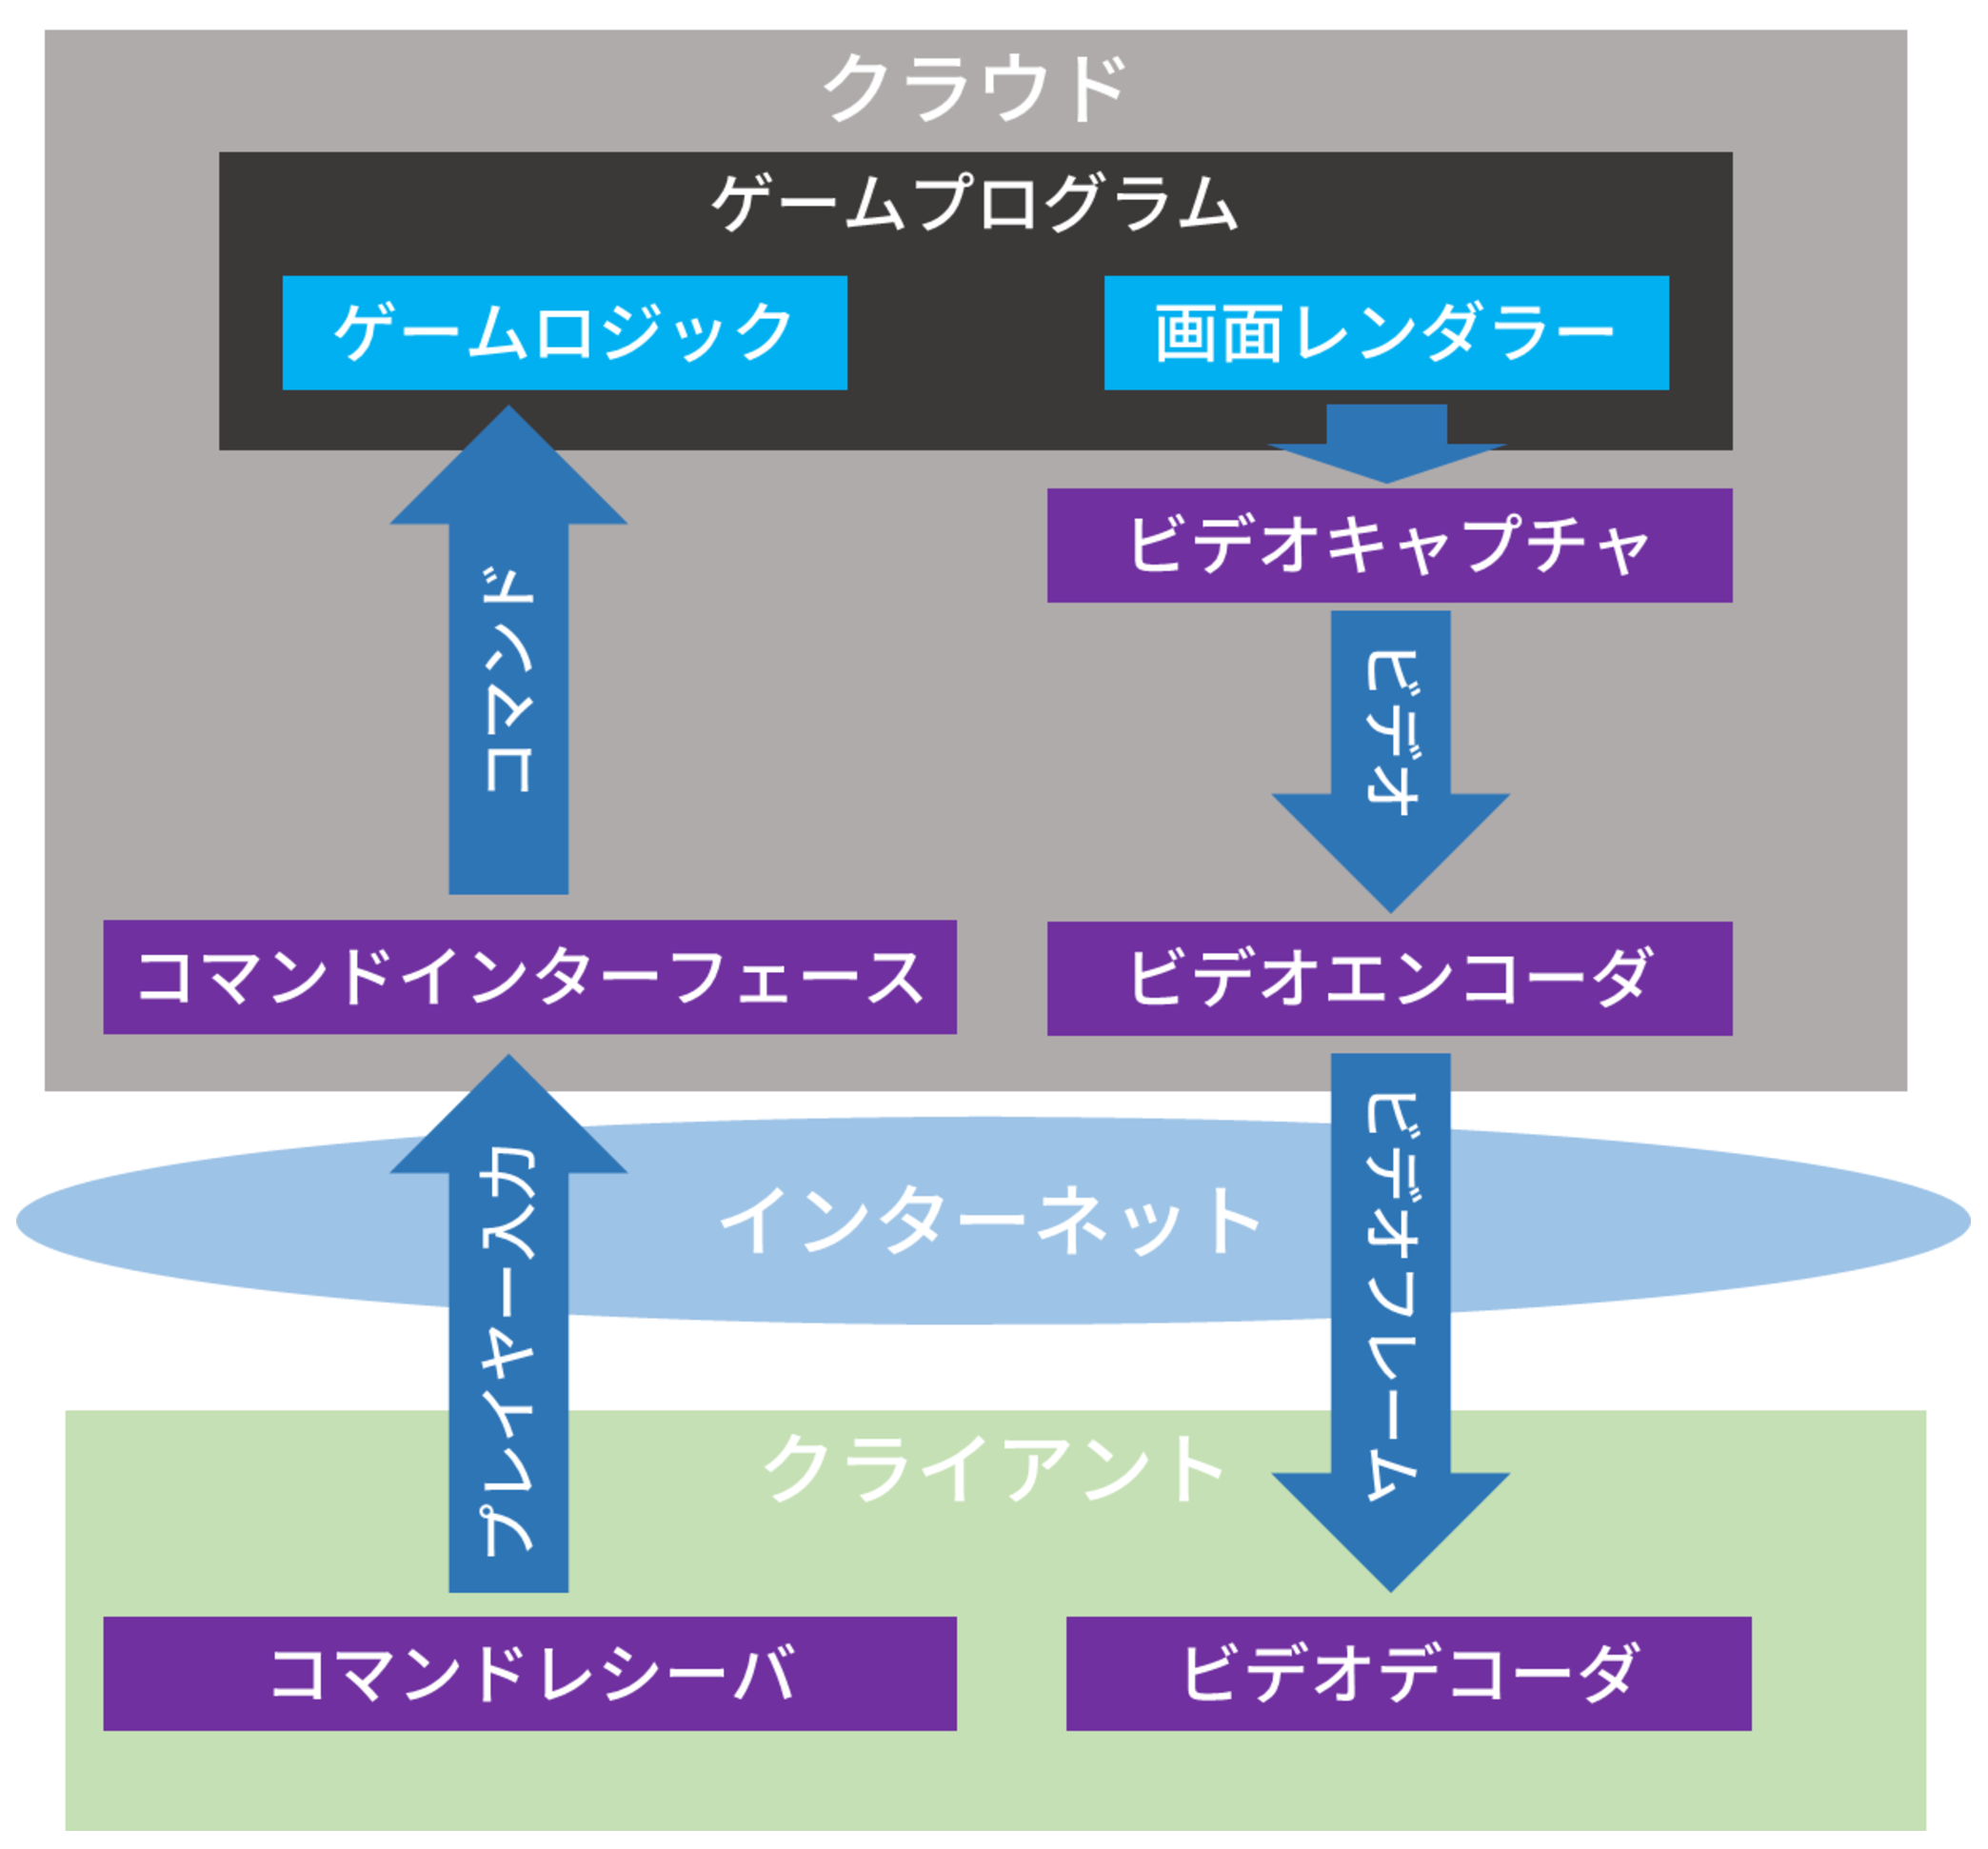
\includegraphics[width=0.8\textwidth,keepaspectratio,clip]{img/cloudgaming.eps}
    \caption{クラウドゲーミングシステム}
    \label{fig:cloudgaming}
\end{figure*}

クラウドゲーミングは商用のサービスの展開もある。過去には英国のOnLive\cite{onlive}やアメリカのGaikaiがクラウドゲーミングサービスを展開していた。これらは既にサービスを終了しているが、ソニーが2012年にGaikaiを買収し、2015年にサービスを閉鎖したOnLiveの資産を取得した\cite{onlive-sony-gaikai}。同年に、ソニーは新たにクラウドゲーミングサービスのPlayStation Now\cite{ps-now}を開始した。また、Googleも2019年にクラウドゲーミングサービスであるGoolge Stadia\cite{stadia}を開始した。同社のウェブブラウザであるGoogle Chromeをインターフェースとしているのが特徴で、ユーザーへのメディアのストリーミングに動画配信サービスのYouTubeを使用している。現在は日本を含まない14カ国で展開されている。また、グラフィックプロセッシングユニットのメーカーとして知られるNVIDIAが提供するクラウドゲーミングサービスGeForce NOW\cite{geforce-now}は、従来PCゲームをプレイしていたプレイヤーをメインターゲットに据えており注目されている。他に、MicrosoftのProject xCloudやAmazonのLunaが海外でサービス開始されている。

商用サービスだけでなく、研究開発用のクラウドゲーミングプラットフォームも存在する。Huangら\cite{gaminganywhere}は、既存のクローズドソースのシステムではクラウドゲーミングを体験するためのテストベッドの設置が困難であることから、オープンソースのクラウドゲーミングプラットフォームであるGamingAnywhereを開発した。GamingAnywhereはWindows、Linux、OS X上で実装されており、クライアントはiOSやAndroid等の他のOSにも移植が可能である。また、GamingAnywhereは詳細な設定を可能にしていて、更にオープンソースであるため拡張的な実装が可能であるなど、クラウドゲーミングのシステム研究のテストベッドの構築に適している。

従来のゲームシステムとは一線を画するクラウドゲーミングには、依然として重要な課題が存在している\cite{cloudgaming-survey}。クラウドゲーミングプロバイダの立場から見た課題としては、ゲーム環境の仮想化やサーバにおける負荷分散などといった課題がある。一方、システムのユーザーであるプレイヤーが知覚するゲーム体験の品質の評価指標であるQuality of Experience(QoE)
を確保することも重要な課題である。クラウドゲーミングのプレイにおけるQoEの確保に必要な課題の構成要素としては、以下のようなものがある。
\begin{itemize}
    \item ストリーミングされるゲーム画面の高品質な画質の担保
    \item ゲーム画面のリアルタイムストリーミングに耐えうる、充分なネットワーク帯域の確保
    \item 伝送データ圧縮や効率的なストリーミング技術
    \item プレイヤー端末での画面表示やプレイヤーによる操作が画面に反映されるまでの遅延の最小化
\end{itemize}

中でもプレイヤーの操作に対する応答性に直結する遅延の問題は重要である。動画配信プラットフォームにおけるライブストリーミングの場合、途切れることなく安定した動画の配信を行うためにバッファリングを行うことで対処する場合がある。しかしクラウドゲーミングは多くの場合、リアルタイムかつインタラクティブな性質を持つコンテンツであるためこの方法を使用することができない。そのため、クラウドサーバ上でのゲーム画面生成の高速化/効率化や、伝送データの圧縮、ネットワーク遅延の最小化などが課題となっている。

クラウドのデータセンターは、通常国内には数箇所しか設置されていない。このため、データセンターに地理的に遠いプレイヤーの端末から接続するとネットワーク遅延が大きくなってしまうという問題がある。データセンターに計算機資源を集約する現在のクラウドアーキテクチャを利用する限り、この遅延を解消することはできない。プレイヤーとクラウド上の計算機資源との間の物理的距離に起因する遅延の問題解決するためには、プレイヤーの近傍に計算機資源を設置することが必要である。

ところで、多量のタスクを小規模なタスクに分割して、ボランティアの提供する多数のコンピュータリソースに広域に分散して処理するボランティアコンピューティングという枠組みがある。SETI@home\cite{setiathome}やFolding@home\cite{folding}に代表されるボランティアコンピューティングプロジェクトが、高エネルギー物理学、分子生物学、医学、天体物理学、気候研究などの分野の研究で利用された。クラウドコンピューティングの枠組みにおいては、クラウドサーバに一極集中したリソースにユーザがアクセスして利用する。それに対し、ボランティアコンピューティングにおいては、広域に分散した一般ユーザーのリソースを活用するという特徴がある。国内に数箇所しか設置されていないクラウドのデータセンターに比べて、広域に分散した一般ユーザーのリソースは地理的に近傍である可能性が高い。この性質を利用し、よりネットワーク遅延の小さい計算機同士での通信でクラウドゲーミングを行えば、遅延の問題を解消する可能性がある。

本研究では、ボランティアが提供する地理的に近傍の遊休コンピュータのリソースを活用することによるクラウドゲーミングシステムを提案する。既存のクラウドゲーミングアーキテクチャにおいては、クラウドのデータセンターでゲームが動作しているために、プレイヤーの端末からデータセンターまでのネットワーク遅延を回避することは不可能である。国内のデータセンターまでのネットワーク遅延は最大50ms程度と言われている(出典がない)。これはゲームプレイにおけるレスポンスの遅延としては無視できない値であり、著しくプレイヤーのQoE低下の原因となり得る。本研究では、プレイヤーの端末からデータセンターまでのネットワーク遅延を削減し、プレイヤーがクラウドゲーミングのプレイを通して体験する画面表示や操作の反映の遅延を最小化することでのプレイヤーのQoEの向上を目的とする。広域に分散したボランティアの提供する遊休コンピュータの中から、プレイヤーの端末から見て地理的に近傍のものを選択し、その上でクラウドゲームサーバを動作させる。これによって遅延の削減を目指す。

本論文の以後の部分は次のように構成されている。2章では、研究分野の背景、関連研究について述べる。3章では、提案システムの設計について述べる。4章では、提案システムの実装について述べる。5章では、提案システムの性能評価について述べる。6章では、まとめと今後の展望について述べる。







 


\newpage
\section{現状と今後の課題}
\label{kadai}

現状と今後の課題 現状と今後の課題 現状と今後の課題 現状と今後の課題 
現状と今後の課題 現状と今後の課題 現状と今後の課題 現状と今後の課題 
現状と今後の課題 現状と今後の課題 現状と今後の課題 現状と今後の課題 
現状と今後の課題 現状と今後の課題 現状と今後の課題 現状と今後の課題 

現状と今後の課題 現状と今後の課題 現状と今後の課題 現状と今後の課題 
現状と今後の課題 現状と今後の課題 現状と今後の課題 現状と今後の課題 
現状と今後の課題 現状と今後の課題 現状と今後の課題 現状と今後の課題 
現状と今後の課題 現状と今後の課題 現状と今後の課題 現状と今後の課題 

現状と今後の課題 現状と今後の課題 現状と今後の課題 現状と今後の課題 
現状と今後の課題 現状と今後の課題 現状と今後の課題 現状と今後の課題 
現状と今後の課題 現状と今後の課題 現状と今後の課題 現状と今後の課題 
現状と今後の課題 現状と今後の課題 現状と今後の課題 現状と今後の課題 

%
% 謝辞
%
\acknowledgements
ありあとやす
%
% 参考文献
% ここでは \reference を使って、自分でリストを作るか、BibTeX を使って
% リストをつくって下さい。この例では BibTeX を作るような形式になってい
% ます。
%
\newpage
% \reference
\bibliographystyle{plain}
\bibliography{mthesis}
%
% 付録
%
\appendix

\section{おまけその1}
\label{omake1}

これはおまけです。これはおまけです。これはおまけです。これはおまけです。
これはおまけです。これはおまけです。これはおまけです。これはおまけです。
これはおまけです。これはおまけです。これはおまけです。これはおまけです。
これはおまけです。これはおまけです。これはおまけです。これはおまけです。

\begin{figure}
\centerline{これはおまけの図です。}
\caption{おまけの図}
\end{figure}


\section{おまけその2}

これもおまけです。これもおまけです。これもおまけです。これもおまけです。
これもおまけです。これもおまけです。これもおまけです。これもおまけです。
これもおまけです。これもおまけです。これもおまけです。これもおまけです。
これもおまけです。これもおまけです。これもおまけです。これもおまけです。

\end{document}

